\subsection{Creating NCAP test scenario CPNC-50}
A major part of the project deals with the used software to create the test environment and the test scenario itself. With its variable sensor suites and full controllable static and dynamic actors an maps CARLA is especially suitable for setting up an own test scenario \cite{Dosovitskiy17}. The adaptable \ac{API} and the \ac{ROS} integration provides a lot of flexibility and the possibility to extract the \ac{GT} data directly from the scenario. The work is based on CARLA 0.9.8 release combined with \ac{ROS} melodic which uses python3 packages and an \ac{API} based on python3.5. The test case is derived from the Euro NCAP autonomous emergency braking scenario which uses the Car-to-Pedestrian Nearside Child 50\,\% (CPNC-50) test case from the Insurance Institute for Highway Safety (IIHS) test protocol \cite{NCAP, Protocoll}. \Cref{Test conditions} presents the elementary test conditions for the created test scenario. 

\begin{table}[h]
	\caption{Test conditions pedestrian autonomous emergency braking (P-AEB) \cite{Protocoll}}
	\label{Test conditions}
	\begin{center}
		\begin{tabular}{l l}
			\hline
			Parameter & CPCN-50 Scenario Child\\
			\hline
			Test vehicle speed & 40 km/h\\
			Pedestrian target speed & 5 km/h\\
			Target direction        & Crossing from R-to-L\\
			Target path             & Perpendicular\\
			Pedestrian dummy size   & Child\\
			Overlap                 & 50 \%\\
			\hline
			
			
		\end{tabular}
	\end{center}
\end{table}


\begin{figure}[H]
	\centering
	\fbox{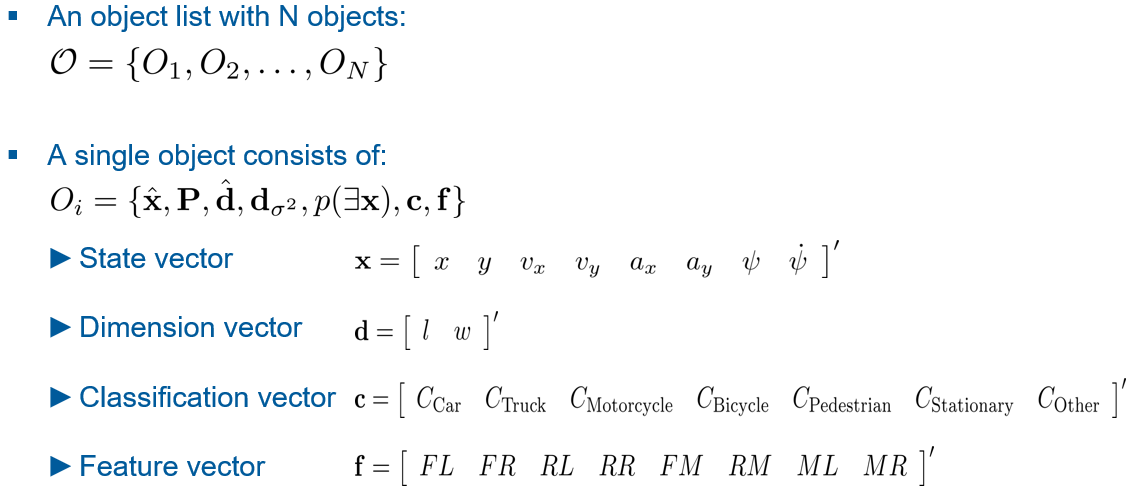
\includegraphics[width=1\linewidth]{vector.png}}
	\caption{Object list vector \cite{Aeberhard}}
	\label{fig:vectors}
\end{figure}

	
\begin{figure*}[]
	\centering
	\fbox{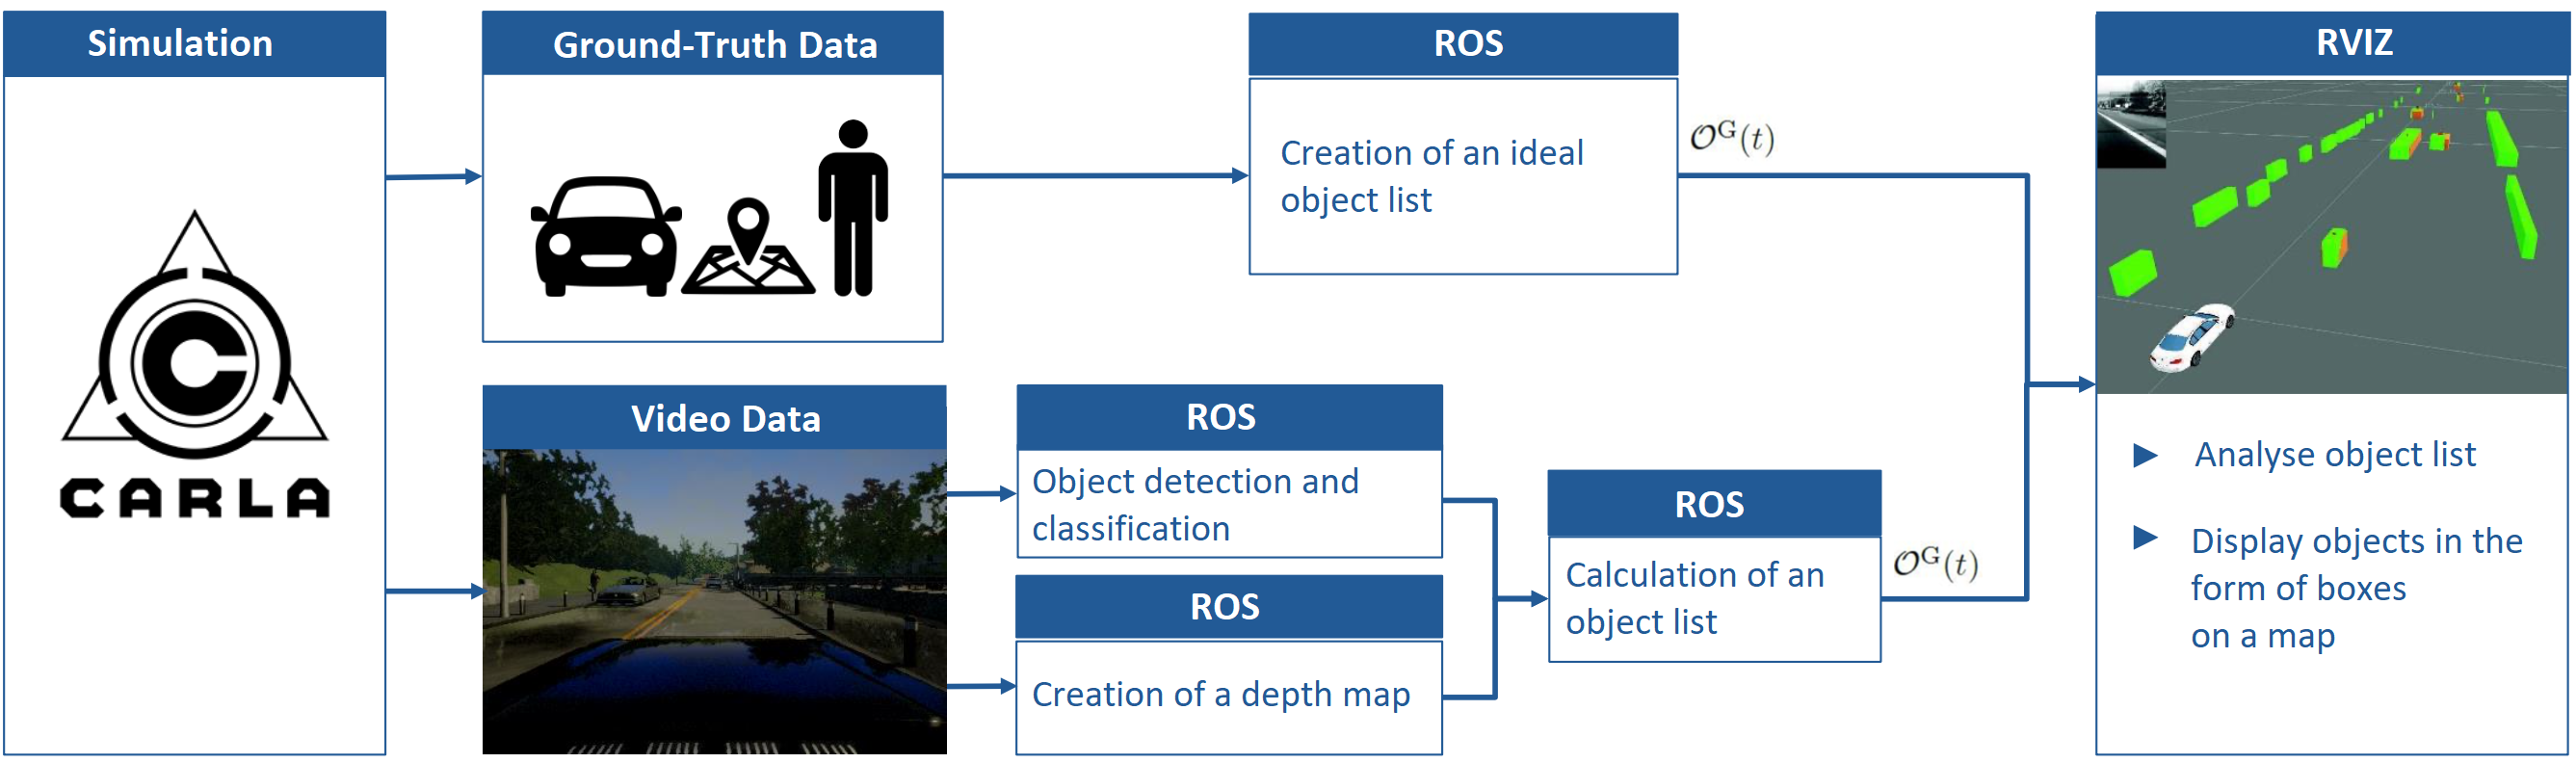
\includegraphics[width=0.85\linewidth]{Overview}}
	\caption{Process diagram for data generation, illustration and evaluation}
	\label{fig:Overview}
\end{figure*}

The test procedure starts with launching the test scenario by first spawning the three vehicles and the pedestrian to their initial positions into the map. This state consists of an Audi TT (1) in front and an Audi e-tron (2) arranged behind it. The left edges of both cars are parked 0.2 m away from the right edge of the test lane. The longitudinal distance between the cars and between the front car and pedestrian is 1.0 m, each. At the beginning of the simulation, the child is positioned 7.0 m laterally from the center of the ego-vehicle, which is centered in its lane 200 m behind the pedestrian and portrayed as an Audi e-tron. A few seconds after spawning, the ego-vehicle starts accelerating quickly to 40 km/h and the child starts moving with constant speed of 5 km/h from right-to-left to cross the street. The pedestrian becomes visible for the ego-vehicle after he passed the Audi e-tron (2). \Cref{fig:coordination} illustrates the positioning of all vehicles and the pedestrian at this time.

The ego-vehicle immediately engages an emergency brake and comes to a standstill in front of the child. At this point the pedestrian is at the 50\,\% overlapping point. The child continues crossing the street and the scenario ends as soon as the child completely passed the ego-vehicle.
\begin{figure}[b]
	\centering
	\fbox{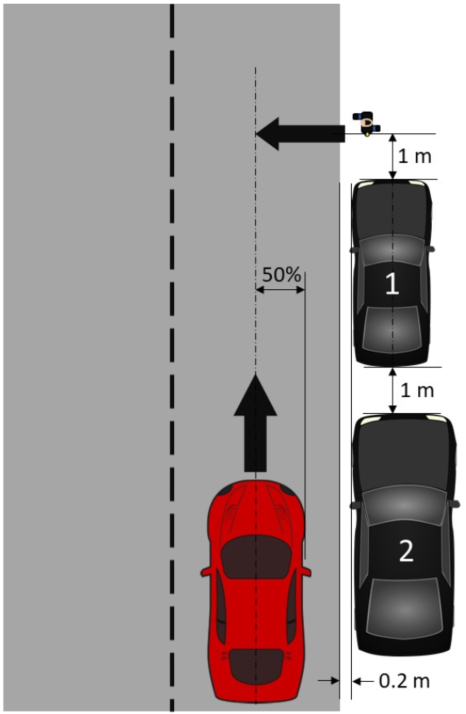
\includegraphics[width=0.23\textwidth]{images/Target_Placement_test_scenario.png}}
	\caption{Target placement based on CPNC-50 Scenario Child \cite{Protocoll}}
	\label{fig:coordination}
\end{figure}

\begin{figure}[b]
	\centering
	\fbox{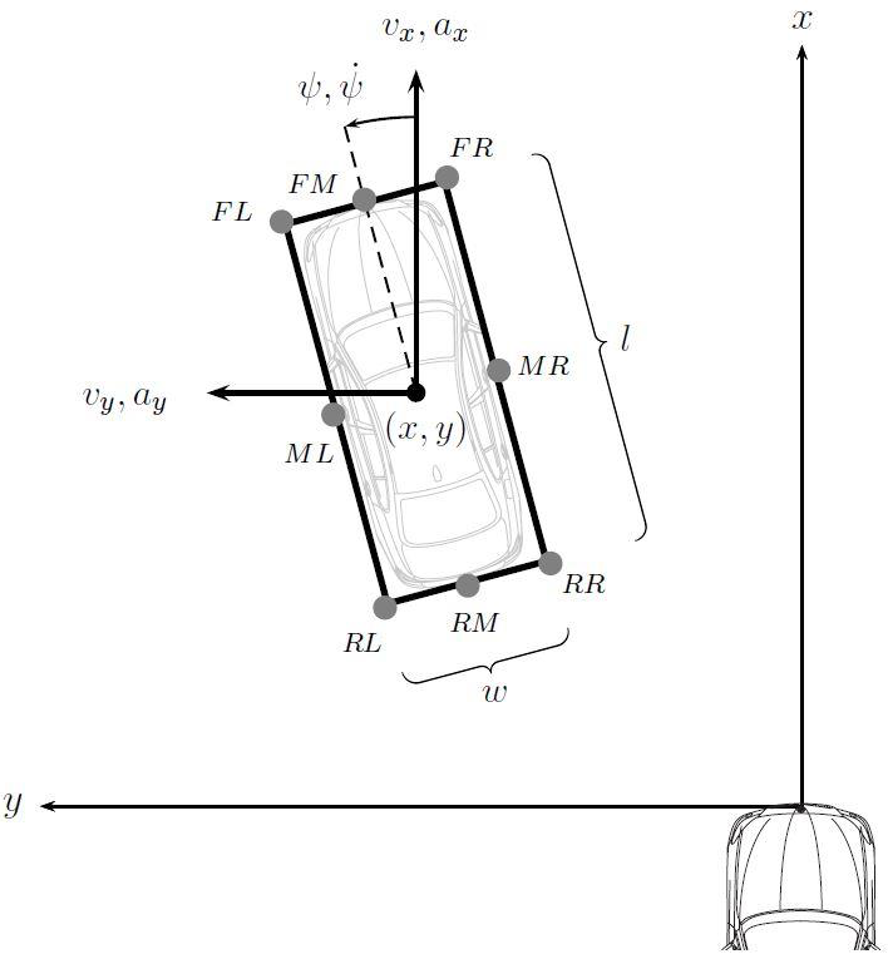
\includegraphics[width=0.8\linewidth]{images/KoordinatenSystem}}
	\caption{Vehicle and pedestrian coordinate system \cite{Aeberhard}}
	\label{fig:coordinate}
\end{figure}
\subsection{Creating objects list of \ac{GT} data}\label{B}
The \ac{GT} Objects List includes four message vectors for every spawned object-,Classification, Dimension, Features and Geometric shown in \cref{fig:vectors}. These messages are used to classify the objects, send their geometrical dimensions, location, acceleration, angles and visible edges \cite{Aeberhard}.
The Classification parameters indicate the type of the spawned objects and differentiate between the relevant classes car and pedestrian. In addition, the Features vector contains all visible and invisible edges of the objects. The evaluation of both messages is statically generated for this scenario referring to the bounding box data of every spawned object. The third message represents the length, width and height of the object. This Dimensions vector receives the information as well from the bounding box. Furthermore, the Geometric message is used to represent the coordinates, velocity, yaw angle and acceleration of the objects relative to the ego-vehicle. 
The \ac{GT} data will be published via \ac{ROS} in two different topics. Every topic includes a header with timestamp, object \ac{ID} as well as an Objects List message. This message includes all four messages vectors mentioned before for the pedestrian and both parked vehicles in topic one and is referenced to the center of the objects. \Cref{fig:coordinate} illustrates the coordinate system used for the ego-vehicle (bottom right) and the two parked vehicles and the pedestrian (center). 

Topic two includes only the Objects List message with the Geometric data of the ego-vehicle based on the camera position at the front middle of the ego-vehicle.
The test scenario offers two options for publishing different data in topic one.
\begin{itemize}
	\item Publishing only objects in the field of view of the camera (200 m and a total opening angle of \ang{60})
	\item Publishing all spawned objects over the whole test period
\end{itemize}